
%(BEGIN_QUESTION)
% Copyright 2006, Tony R. Kuphaldt, released under the Creative Commons Attribution License (v 1.0)
% This means you may do almost anything with this work of mine, so long as you give me proper credit

Billøftere brukt i verksteder drives ofte av et «olje under lufttrykk»-system. Trykkluft fra verkstedets kompressor (brukt til håndverktøy, pumping av dekk, rengjøring av deler osv.) er lett tilgjengelig og kan brukes som trykkilde for en løftesylinder med stempel. Ved å bruke trykkluft trengs det ikke en separat hydraulikkpumpe for å bygge trykk i oljen som brukes i sylinderen:

$$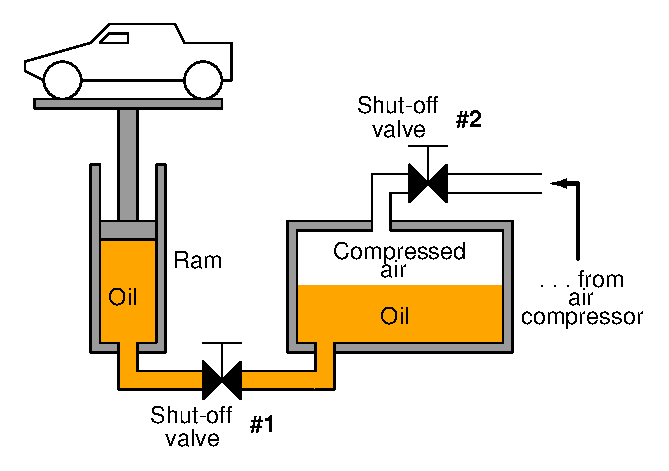
\includegraphics[width=15.5cm]{i00751x01.eps}$$

Hvilken stengeventil er tryggest å lukke for å stoppe plattformens oppadgående bevegelse når en bil løftes fra bakken? Hvorfor?

\vskip 10pt

Hvis du fikk ansvar for vedlikehold på denne løfteren, hvordan ville du brukt standard «lock-out, tag-out»-prosedyrer for å sikre en tilstand med {\it null energi}? Hvor ville du satt låser og merkelapper, og i hvilke posisjoner må disse sikkerhetsenhetene stå før låsing/merking utføres?

\vskip 20pt \vbox{\hrule \hbox{\strut \vrule{} {\bf Forslag til sokratisk diskusjon} \vrule} \hrule}

\begin{itemize}
\item{} Stempeltetninger lekker, og kan i verste fall svikte katastrofalt. Beskriv virkningene av slik tetningssvikt i denne billøfteren, og angi hvordan systemet kan gjøres sikkert for mekanikeren hvis dette skjer.
\item{} Angi hvor eventuelle ekstra ventiler kan plasseres i systemet for å gjøre lockout til nullenergitilstand enklere.
\item{} Er størrelsen på luft/olje-reservoaret en faktor for løfterens maksimale løftekapasitet? Hvorfor eller hvorfor ikke?
\item{} Er størrelsen på stempelarealet i sylinderen en faktor for løfterens maksimale løftekapasitet? Hvorfor eller hvorfor ikke?
\item{} Er diameteren på luft- og/eller oljerørene en faktor for løfterens maksimale løftekapasitet? Hvorfor eller hvorfor ikke?
\item{} I systemer der flere enheter må låses ut før vedlikehold, er det vanlig å bruke en {\it lock box} med låser og nøkler for alle enhetene, og så lar man hver vedlikeholdsarbeider sette sin personlige hengelås på lokket slik at boksen ikke kan åpnes. Forklar hvordan et slikt «lock-box»-system holder alle trygge.
\end{itemize}

\underbar{file i00751}
%(END_QUESTION)





%(BEGIN_ANSWER)

Stengeventil \#1 (oljeventilen) er den tryggeste å lukke for å stoppe plattformens vertikale bevegelse.

%(END_ANSWER)





%(BEGIN_NOTES)

Stengeventil \#1 (oljeventilen) er den tryggeste å lukke for å stoppe plattformens vertikale bevegelse. Når denne ventilen er lukket, blir plattformen hydraulisk «låst» i posisjon, og kan ikke bevege seg verken opp eller ned selv om det påføres ytre krefter.

\vskip 10pt

Hvis stengeventil \#2 lukkes mens ventil \#1 står åpen, stopper plattformen riktignok å stige, men den kan fortsatt bevege seg opp og ned ved ytre påvirkning. Hvis en mekaniker for eksempel drar i plattformen, kan den bevege seg litt når bare ventil \#2 er lukket.

\vskip 10pt

Forskjellen mellom konsekvensene av å stenge den ene eller den andre ventilen skyldes oljens {\it inkompressibilitet} og luftens {\it kompressibilitet}.

\vskip 10pt

For øvrig brukes også mekaniske «chocks» for å sikre en løftet bil i høyden etter løfting. Mekanikere stoler med god grunn ikke bare på sylinderen til å holde bilens vekt, siden stempeltetninger kan lekke og noen ganger svikte katastrofalt!

\vfil \eject

\noindent
{\bf Oppsummeringsquiz:}

Hvilken stengeventil er tryggest å lukke for å hindre at plattformen beveger seg etter at en bil er løftet opp fra bakken? Hvorfor?

$$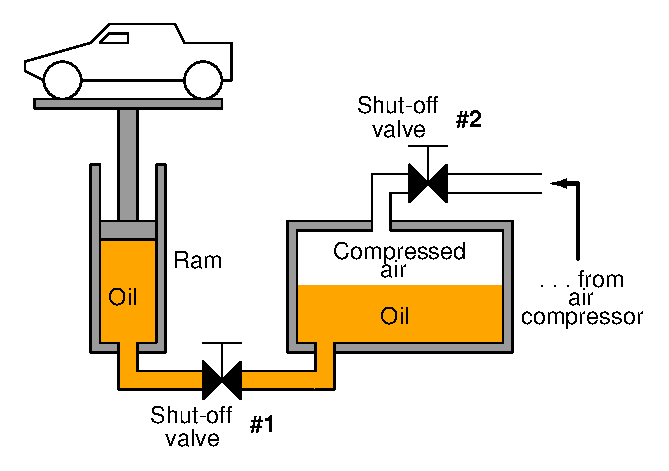
\includegraphics[width=15.5cm]{i00751x01.eps}$$

\begin{itemize}
\item{} Ventil \#2, fordi luftens kompressibilitet «låser» bilen i posisjon
\vskip 5pt
\item{} Ventil \#1, fordi oljens inkompressibilitet «låser» bilen i posisjon
\vskip 5pt
\item{} Ventil \#1, fordi dette hindrer stempellekkasje i å senke bilen
\vskip 5pt
\item{} Ventil \#2, fordi dette hindrer lekkasje i luft/olje-reservoaret i å senke bilen
\vskip 5pt
\item{} Ventil \#1, fordi lukking av ventil \#2 vil overbelaste luftkompressoren
\vskip 5pt
\item{} Ventil \#2, fordi dette bidrar til å hindre forurensning av oljen fra vann i luften
\end{itemize}


%INDEX% Mekanikk, fluidkraftsystemer: hydraulisk/pneumatisk billøfter
%INDEX% Fysikk, statiske væsker: kompressibilitet
%INDEX% Prosess: hydraulisk billøfter
%INDEX% Sikkerhet, lock-out / tag-out: korrekt prosedyre

%(END_NOTES)


